\documentclass[12pt,a4paper]{article}
\usepackage[utf8]{inputenc}
\usepackage[spanish,es-tabla]{babel}
\usepackage{geometry}
\usepackage{graphicx}
\usepackage{multirow}
\usepackage{tabularx}
\usepackage{mathptmx}
\usepackage{fancyhdr}
\usepackage{array}
\usepackage[table]{xcolor}
\usepackage{titlesec}
\usepackage{setspace}
\usepackage{microtype}
\usepackage{lastpage}
\usepackage{booktabs}
\usepackage{enumitem}
\usepackage{amsmath}
\usepackage{amsfonts}
\usepackage{amssymb}

\graphicspath{{images/}{../images/}{./}}

\geometry{
    top=4.7cm,
    bottom=2.5cm,
    left=2.5cm,
    right=2.5cm,
    headheight=3.9cm,
    headsep=0.4cm
}

\setstretch{1.15}
\setlength{\parindent}{0pt}
\setlength{\parskip}{0.45em}
\setlength{\tabcolsep}{4pt}

\titleformat{\section}
  {\normalfont\fontsize{12}{14.5}\bfseries}{\thesection.}{0.6em}{\uppercase}
\titlespacing*{\section}
  {0pt}{1.8ex plus 0.4ex minus 0.2ex}{0.6ex plus 0.2ex}

\titleformat{\subsection}
  {\normalfont\fontsize{11.5}{13.5}\bfseries}{\thesubsection.}{0.5em}{}
\titlespacing*{\subsection}
  {0pt}{1.4ex plus 0.3ex minus 0.1ex}{0.4ex plus 0.1ex}

\titleformat{\subsubsection}
  {\normalfont\fontsize{10.5}{12.5}\bfseries\itshape}{\thesubsubsection.}{0.4em}{}
\titlespacing*{\subsubsection}
  {0pt}{1.1ex plus 0.2ex minus 0.1ex}{0.3ex plus 0.1ex}

\newcolumntype{Y}{>{\centering\arraybackslash}X}
\newcolumntype{L}{>{\raggedright\arraybackslash}X}
\newcolumntype{C}{>{\centering\arraybackslash}X}

\definecolor{headerblue}{RGB}{26, 54, 93}
\definecolor{darkblue}{RGB}{43, 108, 176}
\definecolor{lightgraybg}{RGB}{248, 248, 248}
\definecolor{tableheader}{RGB}{232, 238, 246}

\newcommand{\docCodigo}{TI-SIGE-ENT-F2-005}
\newcommand{\docVersion}{1.0}
\newcommand{\docProceso}{EXPERIENCIA DE USUARIO / WIREFRAMES UI-UX}
\newcommand{\docElaboracion}{03/09/2026}
\newcommand{\docRevision}{03/09/2026}
\newcommand{\docTitulo}{DISEÑO DE INTERFACES Y EXPERIENCIA DE USUARIO}
\newcommand{\docOrganizacion}{FACULTAD DE INGENIERÍA EN SISTEMAS, ELECTRÓNICA E INDUSTRIAL}
\newcommand{\docSubOrganizacion}{CARRERA DE INGENIERÍA DE SOFTWARE}

\newcommand{\encabezadofrecuente}{%
    \renewcommand{\arraystretch}{1.15}%
    \noindent\makebox[\textwidth][c]{%
    \begin{tabularx}{\textwidth}{|>{\centering\arraybackslash}m{2.8cm}|Y|>{\centering\arraybackslash}m{4.8cm}|}
        \hline
        \multirow{4}{2.8cm}{\centering\raisebox{-1.15cm}{
\includegraphics[width=2.5cm,height=2.0cm,keepaspectratio]{images/logo.png}}}
        & \textbf{\fontsize{9}{11}\selectfont \docOrganizacion} 
        & \textbf{\fontsize{8}{10}\selectfont CÓDIGO:} \fontsize{8}{10}\selectfont \docCodigo \\
        \cline{3-3}
        & \textbf{\fontsize{8.5}{10.5}\selectfont \docSubOrganizacion} 
        & \textbf{\fontsize{8}{10}\selectfont VERSIÓN:} \fontsize{8}{10}\selectfont \docVersion \\
        \cline{2-3}
        & \textbf{\fontsize{8}{10}\selectfont PROCESO:} \fontsize{8}{10}\selectfont \docProceso 
        & \textbf{\fontsize{8}{10}\selectfont ELABORACIÓN:} \fontsize{8}{10}\selectfont \docElaboracion \\
        \cline{2-3}
        & \textbf{\fontsize{8.5}{10.5}\selectfont \docTitulo} 
        & \textbf{\fontsize{8}{10}\selectfont ÚLTIMA REVISIÓN:} \fontsize{8}{10}\selectfont \docRevision \\
        \hline
    \end{tabularx}%
    }%
}

\pagestyle{fancy}
\fancyhf{}
\fancyhead[C]{\encabezadofrecuente}
\fancyfoot[C]{\fontsize{10}{12}\selectfont Página \thepage\ de \pageref{LastPage}}
\renewcommand{\headrulewidth}{0pt}

\begin{document}

\noindent{\fontsize{10.5}{12.5}\selectfont \textbf{Integrantes:} Heidi Villavicencio \quad$\vert$\quad Steeven Toala \quad$\vert$\quad Nixon Hurtado \quad$\vert$\quad Andrea Vásquez}

\vspace{0.25cm}

\section{Título}
\textbf{Denominación del Entregable:} Diseño de Interfaces y Experiencia de Usuario (Wireframes y UX) -- Código EDT: 2.5

\section{Introducción}
La usabilidad y la experiencia de usuario (UX) son determinantes para la adopción exitosa del software en entornos universitarios. El cuerpo docente requiere una interfaz moderna, limpia y predecible que minimice la fatiga visual y agilice el registro de sus labores. Este informe consolida el diseño de alta fidelidad, la arquitectura de interfaces, el flujo del Wizard modular de 4 pasos para el elaborador, los componentes de la matriz interactiva y el panel de revisión colegiada, acompañados de una guía de estilos y tokens cromáticos institucionales accesibles bajo el estándar WCAG 2.1 nivel AA.

\section{Objetivo}
\subsection{Objetivo General}
Diseñar la arquitectura de interfaces y experiencia de usuario (UI/UX) del sistema SIGE, elaborando wireframes de alta fidelidad, flujos interactivos y el sistema de diseño accesible.
\subsection{Objetivos Específicos}
\begin{itemize}[leftmargin=1.5em, itemsep=2pt]
    \item Diseñar el Wizard modular de 4 pasos para la elaboración secuencial de documentos.
    \item Maquetar la Matriz Dinámica responsive que replica la Tabla 1 del formato SGC.
    \item Diseñar el panel de revisión del Comité con bandeja de observaciones contextuales.
    \item Establecer la paleta de colores institucional, tipografía y tokens accesibles WCAG AA.
\end{itemize}

\section{Alcance}
\subsection{Límites del Entregable (In-Scope)}
\begin{itemize}[leftmargin=1.5em, itemsep=2pt]
    \item Vistas de Dashboard Docente, Editor Wizard, Tabla de Matriz, Subida de Archivos y Panel de Revisión.
    \item Prototipo interactivo en Figma y especificación de tokens para Tailwind CSS.
\end{itemize}
\subsection{Exclusiones (Out-of-Scope)}
\begin{itemize}[leftmargin=1.5em, itemsep=2pt]
    \item Código JavaScript de componentes React (cubierto en Fase 3).
\end{itemize}

\section{Definiciones}
\begin{itemize}[leftmargin=1.5em, itemsep=2pt]
    \item \textbf{Wireframe de Alta Fidelidad:} Representación visual interactiva y detallada de la interfaz con colores y tipografías reales.
    \item \textbf{Design Tokens:} Variables de diseño centralizadas (colores, espaciados, fuentes) que garantizan consistencia visual.
    \item \textbf{WCAG 2.1 (Nivel AA):} Pautas de Accesibilidad para el Contenido Web con ratios mínimos de contraste cromático (4.5:1).
    \item \textbf{Wizard de Navegación:} Patrón de diseño UI que guía al usuario paso a paso a través de un flujo complejo.
\end{itemize}

\section{Responsabilidades}
\begin{itemize}[leftmargin=1.5em, itemsep=2pt]
    \item \textbf{Heidi Villavicencio / Andrea Vásquez (Responsables EDT 2.5):} Diseño UI en Figma, investigación de usuarios y diseño del sistema visual.
    \item \textbf{Steeven Toala (Líder Técnico):} Verificación de factibilidad de maquetación en Tailwind CSS.
    \item \textbf{Ing. Paulo Torres (Docente Evaluador):} Aprobación del prototipo de interfaces.
\end{itemize}

\section{Normativa Legal y Técnica}
\begin{itemize}[leftmargin=1.5em, itemsep=2pt]
    \item \textbf{W3C Web Content Accessibility Guidelines (WCAG) 2.1.}
    \item \textbf{ISO 9241-210:2019:} Ergonomics of human-system interaction -- Human-centred design for interactive systems.
\end{itemize}

\section{Método, Políticas y Contenidos}
Se utilizó diseño centrado en el usuario (HCD). En las Figuras \ref{fig:s2_05_views} y \ref{fig:s2_05_palette} se aprecian las vistas principales del sistema y la paleta de colores institucional.

\begin{figure}[htbp]
    \centering
    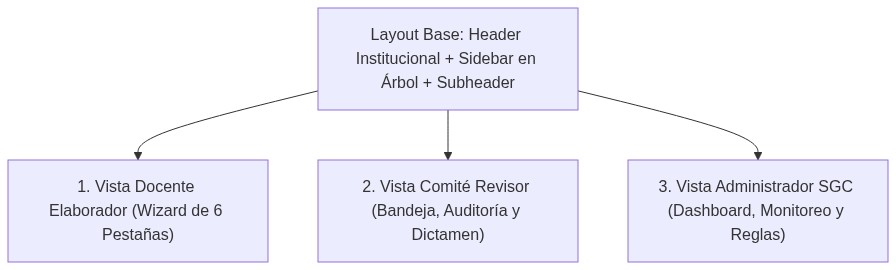
\includegraphics[width=0.88\textwidth,height=5.2cm,keepaspectratio]{images/s2_05_layout_vistas.png}
    \caption{Diseño de Layouts y Vistas del Sistema SIGE.}
    \label{fig:s2_05_views}
\end{figure}

\begin{figure}[htbp]
    \centering
    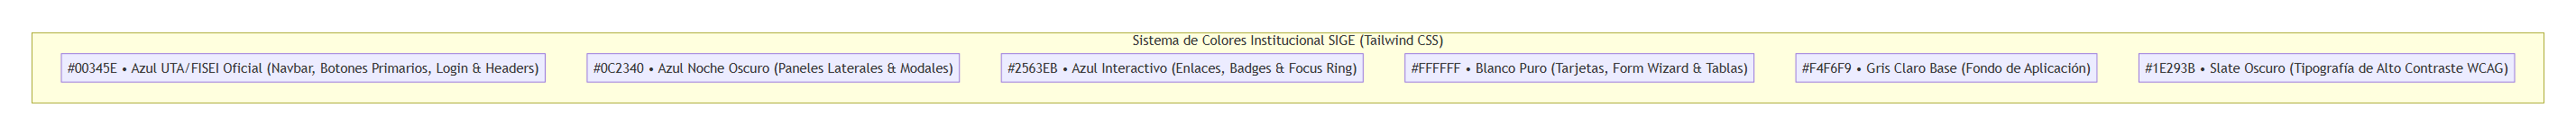
\includegraphics[width=0.80\textwidth,height=5.0cm,keepaspectratio]{images/s2_05_paleta_colores.png}
    \caption{Paleta Cromática y Tokens de Diseño Accesible del Sistema SIGE.}
    \label{fig:s2_05_palette}
\end{figure}

\section{Descripción de actividades}
\subsection{Arquitectura del Wizard Modular de 4 Pasos}
\begin{table}[htbp]
\centering
\small
\renewcommand{\arraystretch}{1.2}
\begin{tabularx}{\textwidth}{|c|>{\bfseries}m{3.2cm}|X|X|}
\hline
\rowcolor{tableheader}
\textbf{Paso} & \textbf{Denominación} & \textbf{Componentes de Interfaz} & \textbf{Validación de Avance} \\
\hline
Paso 1 & Datos Generales & Selección de Período, Dedicación Horaria, Carrera y Asignaturas. & Período activo y datos obligatorios completos. \\
\hline
Paso 2 & Secciones SGC & Editor TipTap con barra de herramientas enriquecida y autoguardado. & Mínimo 50 caracteres por sección requerida. \\
\hline
Paso 3 & Matriz Dinámica & Tabla interactiva de actividades con adición/edición de filas y avance. & Suma estricta de ponderaciones igual a $100.00\%$. \\
\hline
Paso 4 & Resumen y Envío & Visor general de cumplimiento, gestor de evidencias y botón de firma. & Validación de evidencias y ausencia de observaciones. \\
\hline
\end{tabularx}
\caption{Estructura de Pasos del Wizard de Edición.}
\label{tab:wizard_steps}
\end{table}

\subsection{Tokens de Color y Accesibilidad}
La paleta se fundamenta en el azul corporativo institucional:
\begin{itemize}[leftmargin=1.5em, itemsep=2pt]
    \item \textbf{Primary Navy:} \texttt{\#1A365D} (Contraste 11.2:1 con fondo blanco, cumple WCAG AAA).
    \item \textbf{Accent Blue:} \texttt{\#2B6CB0} (Para botones primarios e indicadores de navegación).
    \item \textbf{Success Green:} \texttt{\#2F855A} (Para estado 100\% de ponderación y firmas válidas).
    \item \textbf{Warning Amber:} \texttt{\#C05621} (Para estados de observación pendiente).
    \item \textbf{Danger Red:} \texttt{\#C53030} (Para bloqueos de Validation Gate y sumatorias incorrectas).
\end{itemize}

\section{Firmas de Responsabilidad}

\noindent
\renewcommand{\arraystretch}{1.2}
\begin{tabularx}{\textwidth}{|>{\raggedright\arraybackslash}m{2.9cm}|>{\raggedright\arraybackslash}X|>{\centering\arraybackslash}m{4.6cm}|>{\centering\arraybackslash}m{2.3cm}|}
    \hline
    \rowcolor{tableheader}
    \textbf{ACCIÓN} & \textbf{NOMBRE Y CARGO} & \textbf{FIRMA} & \textbf{FECHA} \\
    \hline
    \textbf{Elaborado por:} & Heidi Villavicencio\newline Analista de Calidad / UI-UX & \parbox[c]{4.4cm}{\centering\vspace{4pt}
\includegraphics[height=1.5cm,width=4.0cm,keepaspectratio]{images/firma_heidi.png}\vspace{4pt}} & 03/09/2026 \\
    \hline
    \textbf{Revisado por:} & Steeven Toala\newline Líder de Proyecto / Arquitecto & \parbox[c]{4.4cm}{\centering\vspace{4pt}
\includegraphics[height=1.5cm,width=4.0cm,keepaspectratio]{images/firma_steveen.png}\vspace{4pt}} & 03/09/2026 \\
    \hline
    \textbf{Aprobado por:} & Ing. Paulo Torres, Mg.\newline Docente Evaluador -- Gestión Proyectos & \parbox[c]{4.4cm}{\centering\vspace{8pt}\textbf{\textcolor{gray!80}{\scriptsize [ PENDIENTE DE APROBACIÓN ]}}\vspace{8pt}} & \textbf{\textcolor{gray!90}{Pendiente}} \\
    \hline
\end{tabularx}

\vspace{0.4cm}

\section{Control de Cambios}

\noindent
\renewcommand{\arraystretch}{1.2}
\begin{tabularx}{\textwidth}{|>{\hsize=0.45\hsize\centering\arraybackslash}X|>{\hsize=1.55\hsize\raggedright\arraybackslash}X|>{\hsize=1.2\hsize\raggedright\arraybackslash}X|>{\hsize=0.8\hsize\centering\arraybackslash}X|}
    \hline
    \rowcolor{tableheader}
    \textbf{Versión} & \textbf{Descripción del cambio} & \textbf{Responsable del cambio} & \textbf{Fecha de aprobación} \\
    \hline
    1.0 & Emisión inicial del entregable según EDT del Tablero Trello & Equipo de Proyecto SIGE & 03/09/2026 \\
    \hline
\end{tabularx}

\vspace{0.4cm}

\section{Anexos}
\begin{itemize}[leftmargin=1.5em]
\item \textbf{Anexo 1:} Enlace y Especificación del Prototipo Interactivo Figma.
\end{itemize}

\end{document}
